\chapter{Ventas}
\label{mod:08-ventas}

\section{Propósito}
\label{sec:08-proposito}

Registra las ventas de la óptica en dos modalidades sobre una misma cabecera (\code{Venta.Tipo}): \textbf{venta directa} de mostrador (productos/servicios de stock inmediato) y \textbf{venta ``a pedido''} óptica (armazón + cristal a medida + tratamientos + laboratorio externo, con receta obligatoria al confirmar). Cubre también presupuestos (la misma entidad \code{Venta} en estado \code{Borrador}), cobro flexible (contado/crédito, métodos combinados), emisión de documento fiscal (recibo simple o factura timbrada con numeración automática) y devoluciones/cambios.

\section{Entidades principales}
\label{sec:08-entidades}

\begin{longtable}{p{6cm}p{10cm}}
\caption{Entidades principales del módulo de Ventas.}
\label{tab:08-entidades}\\
\toprule
\textbf{Entidad} & \textbf{Rol} \\
\midrule
\endfirsthead
\toprule
\textbf{Entidad} & \textbf{Rol} \\
\midrule
\endhead
\bottomrule
\endfoot
\code{Venta} & Cabecera única para venta directa, presupuesto y venta a pedido (\code{Tipo}/\code{Estado}) \\
\code{VentaLinea} & Línea de producto, servicio o lente a pedido (\code{Tipo}) \\
\code{Cliente} & A quién se le vende (nullable = Consumidor Final) --- ver Capítulo~\ref{mod:06-clientes} \\
\code{Cobro} / \code{CobroLinea} & Pago (seña o cuota) con métodos combinados \\
\code{FacturaVenta} / \code{Comprobante} & Los dos documentos fiscales posibles, mutuamente excluyentes \\
\code{Timbrado} & Serie fiscal con numeración correlativa automática. \code{Tipo} (\code{Tipo}\allowbreak \code{Documento}\allowbreak \code{Fiscal}) separa las series de factura y de nota de crédito \\
\code{Devolucion} / \code{DevolucionLinea} & Devolución o cambio de producto post-venta \\
\code{NotaCredito} & Nota de crédito fiscal emitida al confirmar una devolución sobre una venta facturada \\
\code{TrabajoPedido} & El ``pedido óptico'' de una venta a pedido --- detalle completo en el Capítulo~\ref{mod:09-laboratorio} \\
\code{Receta} & Graduación que respalda una venta a pedido --- ver Capítulo~\ref{mod:05-clinica} \\
\code{Servicio} / \code{ServicioTarifa} & Exámenes/servicios con tarifa por profesional o especialidad, vendibles como línea \\
\end{longtable}

Ver diagrama ER completo en el Capítulo~\ref{sec:modelo-datos}, Figura~\ref{fig:er-ventas}.

\section{Reglas de negocio clave}
\label{sec:08-reglas}

\begin{itemize}
  \item \textbf{Precio de línea autocompleta desde \code{Producto.}\allowbreak \code{PrecioVenta}} (derivado por margen, \hyperref[adr:0004]{ADR 0004}) pero queda editable por línea para un ajuste puntual.
  \item \textbf{El cristal a pedido ya no es un \code{Producto} con stock.} Se especifica en el \code{TrabajoPedido} como \code{TipoLente} (diseño, con \code{PrecioBase} que autocompleta el precio) más \code{Tratamiento}s más precio editable. En \code{VentaLinea} esto se representa como \code{Tipo = Lente}, \textbf{sin \code{ProductoId}} --- no descuenta stock. Ver \hyperref[adr:0007]{ADR 0007}.
  \item \textbf{El \code{TrabajoPedido} de una venta a pedido nace en \code{Borrador}} junto al presupuesto, editable libremente y \textbf{sin aparecer en la cola del laboratorio}. Al confirmar la venta, si sigue en \code{Borrador}, se exige asignar laboratorio y pasa a \code{Pendiente}\allowbreak \code{Aprobacion}. Ver \hyperref[adr:0005]{ADR 0005}.
  \item \textbf{Confirmar una venta \code{TrabajoAPedido} exige \code{RecetaId}.} La receta puede ser de una consulta clínica o cargada manualmente para el cliente (receta ``externa'') --- ver Capítulo~\ref{mod:05-clinica}.
  \item \textbf{El cobro está desacoplado del ciclo del laboratorio.} Toda venta confirmada (directa o a pedido) pasa directo a \code{ListaParaCobrar}; el envío/recepción del trabajo en el laboratorio corre en paralelo sin bloquear el cobro. \code{EstadoVenta.}\allowbreak \code{EnProceso} quedó sin uso para ventas nuevas. Ver \hyperref[adr:0006]{ADR 0006}.
  \item \textbf{Documento fiscal: recibo o factura, nunca ambos.} \code{Comprobante} (recibo simple) y \code{FacturaVenta} (factura timbrada) son mutuamente excluyentes sobre la misma \code{Venta}; ambos producen los mismos efectos (egreso de stock por línea de producto más ingreso de caja, \textbf{sin duplicar} si ya hubo cobros previos) y mueven la venta a \code{Comprobante}\allowbreak \code{Emitido}. La emisión es un paso dedicado (\code{Venta}\allowbreak \code{Comprobante}\allowbreak \code{View}), separado de la pantalla de cobro.
  \item \textbf{Numeración de factura automática por timbrado.} Al emitir una factura, el cajero elige un \code{Timbrado} activo y vigente; el backend genera \code{{Establecimiento}-}\allowbreak \code{{PuntoExpedicion}-}\allowbreak \code{{correlativo:D7}} y avanza \code{Timbrado.}\allowbreak \code{UltimoNumero} --- no hay carga manual del número (\code{VentaService}, confirmado en código: \code{Emitir}\allowbreak \code{Factura}\allowbreak \code{Request} solo lleva \code{TimbradoId}, no número/establecimiento manuales).
  \item \textbf{Una devolución sobre una venta facturada emite nota de crédito; no anula la factura.} Al confirmarse la devolución, si la venta se cerró con \code{FacturaVenta} (no con recibo simple) y hay mercadería devuelta, el sistema emite una \code{NotaCredito} por el valor de lo devuelto, desglosado por categoría fiscal --- la factura original queda intacta y la nota la referencia y compensa. La numeración usa un \code{Timbrado} propio de tipo \code{NotaCredito} vigente en la sucursal: si no hay ninguno configurado, la devolución no se puede confirmar.
  \item \textbf{El reintegro de caja y la nota de crédito son montos independientes.} La nota de crédito se emite por el valor de la mercadería (revierte el documento fiscal), mientras que la plata que sale de caja se limita a lo efectivamente cobrado y no anulado de la venta --- en una venta a crédito con seña solo se reintegra lo que el cliente pagó, porque el saldo financiado nunca entró a caja.
  \item \textbf{\code{Servicio}/\code{ServicioTarifa}} permiten un precio distinto por profesional o por especialidad para el mismo servicio (ej.\ examen); \code{GET /api/servicios/{id}/}\allowbreak \code{precio?professionalId=} resuelve el precio aplicable en el momento de armar la línea.
  \item \textbf{El plan de cuotas de una venta a crédito no se materializa como filas.} La venta guarda solo \code{CantidadCuotas} y \code{FrecuenciaCuotasDias}; el monto de cada cuota, cuántas van pagadas, el vencimiento de la próxima y si está vencida se derivan de esos dos campos más los \code{Cobro} registrados. No existe una tabla de cuotas que pueda quedar desincronizada de los cobros reales.
\end{itemize}

\section{Endpoints}
\label{sec:08-endpoints}

Detalle completo en el Apéndice de Referencia de API, § Ventas (\code{VentasController}, \code{Timbrados}\allowbreak \code{Controller}) y § Catálogo/Inventario para \code{Servicios}\allowbreak \code{Controller} (agrupado ahí en el documento por archivo de origen, pero funcionalmente de este módulo). Flujo de estados de \code{Venta} cubierto por: \code{POST /api/ventas} (crea presupuesto/borrador, con bloque opcional \code{TrabajoPedido}) $\rightarrow$ \code{PUT /api/ventas/{id}/confirmar} $\rightarrow$ \code{POST /api/ventas/cobros} (uno o más) $\rightarrow$ \code{POST /api/ventas/{id}/comprobante} \textbf{o} \code{POST /api/ventas/facturas}.

\section{Flujo típico}
\label{sec:08-flujo}

\textbf{Venta a pedido, de presupuesto a comprobante} (dividido en 2 figuras por la cantidad de pasos):

\begin{figure}[htbp]
\centering
\begin{tikzpicture}[node distance=1.4cm]
  \node[actor] (v) at (0,0) {Vendedor};
  \node[actor] (api) at (4,0) {VentasController};
  \node[actor] (svc) at (8.5,0) {VentaService};
  \node[actor] (db) at (13,0) {PostgreSQL};

  \draw[lineavida] (v.south) -- ++(0,-9.5);
  \draw[lineavida] (api.south) -- ++(0,-9.5);
  \draw[lineavida] (svc.south) -- ++(0,-9.5);
  \draw[lineavida] (db.south) -- ++(0,-9.5);

  \draw[mensaje] ($(v.south)+(0,-1)$) -- node[above,font=\scriptsize]{POST /api/ventas (Tipo=TrabajoAPedido)} ($(api.south)+(0,-1)$);
  \draw[mensaje] ($(api.south)+(0,-2)$) -- node[above,font=\scriptsize]{CrearVentaAsync} ($(svc.south)+(0,-2)$);
  \draw[mensaje] ($(svc.south)+(0,-3)$) -- node[above,font=\scriptsize,align=center]{INSERT Venta(Borrador) + VentaLinea(s)\\+ TrabajoPedido(Borrador)} ($(db.south)+(0,-3)$);
  \node[font=\scriptsize\itshape, align=center] at (13,-3.8) {TrabajoPedido en Borrador,\\invisible para el laboratorio};

  \draw[mensaje] ($(v.south)+(0,-5.2)$) -- node[above,font=\scriptsize]{PUT /api/ventas/{id}/confirmar} ($(api.south)+(0,-5.2)$);
  \draw[mensaje] ($(api.south)+(0,-6.2)$) -- node[above,font=\scriptsize]{ConfirmarVentaAsync} ($(svc.south)+(0,-6.2)$);
  \node[font=\scriptsize, align=left] at (8.5,-7) {valida \code{RecetaId} (TrabajoAPedido)\\valida laboratorio asignado};
  \draw[mensaje] ($(svc.south)+(0,-8)$) -- node[above,font=\scriptsize]{UPDATE Venta.Estado=ListaParaCobrar} ($(db.south)+(0,-8)$);
  \draw[mensaje] ($(svc.south)+(0,-8.9)$) -- node[above,font=\scriptsize]{UPDATE TrabajoPedido.Estado=PendienteAprobacion} ($(db.south)+(0,-8.9)$);
\end{tikzpicture}
\caption{Venta a pedido (1/2): creación del presupuesto y confirmación, momento en el que el \texttt{TrabajoPedido} recién entra a la cola del laboratorio (ver Capítulo~\ref{mod:09-laboratorio}).}
\label{fig:seq-venta-a-pedido-1}
\end{figure}

\begin{figure}[htbp]
\centering
\begin{tikzpicture}[node distance=1.4cm]
  \node[actor] (v) at (0,0) {Vendedor};
  \node[actor] (api) at (4,0) {VentasController};
  \node[actor] (svc) at (8.5,0) {VentaService};
  \node[actor] (db) at (13,0) {PostgreSQL};

  \draw[lineavida] (v.south) -- ++(0,-7.5);
  \draw[lineavida] (api.south) -- ++(0,-7.5);
  \draw[lineavida] (svc.south) -- ++(0,-7.5);
  \draw[lineavida] (db.south) -- ++(0,-7.5);

  \draw[mensaje] ($(v.south)+(0,-1)$) -- node[above,font=\scriptsize]{POST /api/ventas/cobros (seña o total)} ($(api.south)+(0,-1)$);
  \draw[mensaje] ($(api.south)+(0,-2)$) -- node[above,font=\scriptsize]{RegistrarCobroAsync} ($(svc.south)+(0,-2)$);
  \draw[mensaje] ($(svc.south)+(0,-3)$) -- node[above,font=\scriptsize]{INSERT Cobro + CobroLinea(s) + MovimientoCaja} ($(db.south)+(0,-3)$);

  \draw[mensaje] ($(v.south)+(0,-4.5)$) -- node[above,font=\scriptsize]{POST .../comprobante (o .../facturas)} ($(api.south)+(0,-4.5)$);
  \draw[mensaje] ($(api.south)+(0,-5.5)$) -- node[above,font=\scriptsize]{EmitirComprobanteAsync / EmitirFacturaAsync} ($(svc.south)+(0,-5.5)$);
  \draw[mensaje] ($(svc.south)+(0,-7.0)$) -- node[above,font=\scriptsize,align=center,fill=white,inner sep=1.5pt]{egreso stock (líneas Producto) + ingreso caja\\si no hubo cobro previo;\\Venta.Estado=ComprobanteEmitido} ($(db.south)+(0,-7.0)$);
\end{tikzpicture}
\caption{Venta a pedido (2/2): cobro y emisión de comprobante/factura. El laboratorio sigue su propio ciclo en paralelo desde que el \texttt{TrabajoPedido} pasa a \texttt{PendienteAprobacion} --- no bloquea ni es bloqueado por el cobro.}
\label{fig:seq-venta-a-pedido-2}
\end{figure}

\section{Vistas de frontend}
\label{sec:08-frontend}

\code{VentasView.vue}, \code{VentasNuevaView.}\allowbreak \code{vue}, \code{PresupuestosView.}\allowbreak \code{vue}, \code{PresupuestoNuevoView.}\allowbreak \code{vue} (wrappers del editor unificado), \code{components/}\allowbreak \code{VentaEditor.}\allowbreak \code{vue} (prop \code{esPresupuesto}, toggle A pedido/Directa), \code{VentaDetalleView.}\allowbreak \code{vue}, \code{VentaCobrarView.}\allowbreak \code{vue}, \code{VentaComprobanteView.}\allowbreak \code{vue}, \code{CobrosPendientesView.}\allowbreak \code{vue}, \code{FacturasVentaView.}\allowbreak \code{vue}, \code{FacturaDetailView.}\allowbreak \code{vue}, \code{TimbradosView.vue}, \code{VentasCierreView.}\allowbreak \code{vue}; componentes \code{components/}\allowbreak \code{RecetaSelector.}\allowbreak \code{vue}, \code{components/}\allowbreak \code{TrabajoOpticoCard.}\allowbreak \code{vue}, \code{components/}\allowbreak \code{ClienteSelector.}\allowbreak \code{vue}, \code{components/}\allowbreak \code{ClienteQuickCreateModal.}\allowbreak \code{vue}, y el composable \code{composables/}\allowbreak \code{optica.}\allowbreak \code{ts} (arma \code{OpticaState} $\rightarrow$ líneas más bloque \code{TrabajoPedido}). Las devoluciones y cambios no tienen vista propia: viven dentro de \code{VentaDetalleView.}\allowbreak \code{vue}, como un modal ``Devolución / Cambio'' desde el que se solicitan y un bloque que lista las ya registradas sobre esa venta.

\section{Interfaz}
\label{sec:08-interfaz}

\begin{figure}[htbp]
\centering
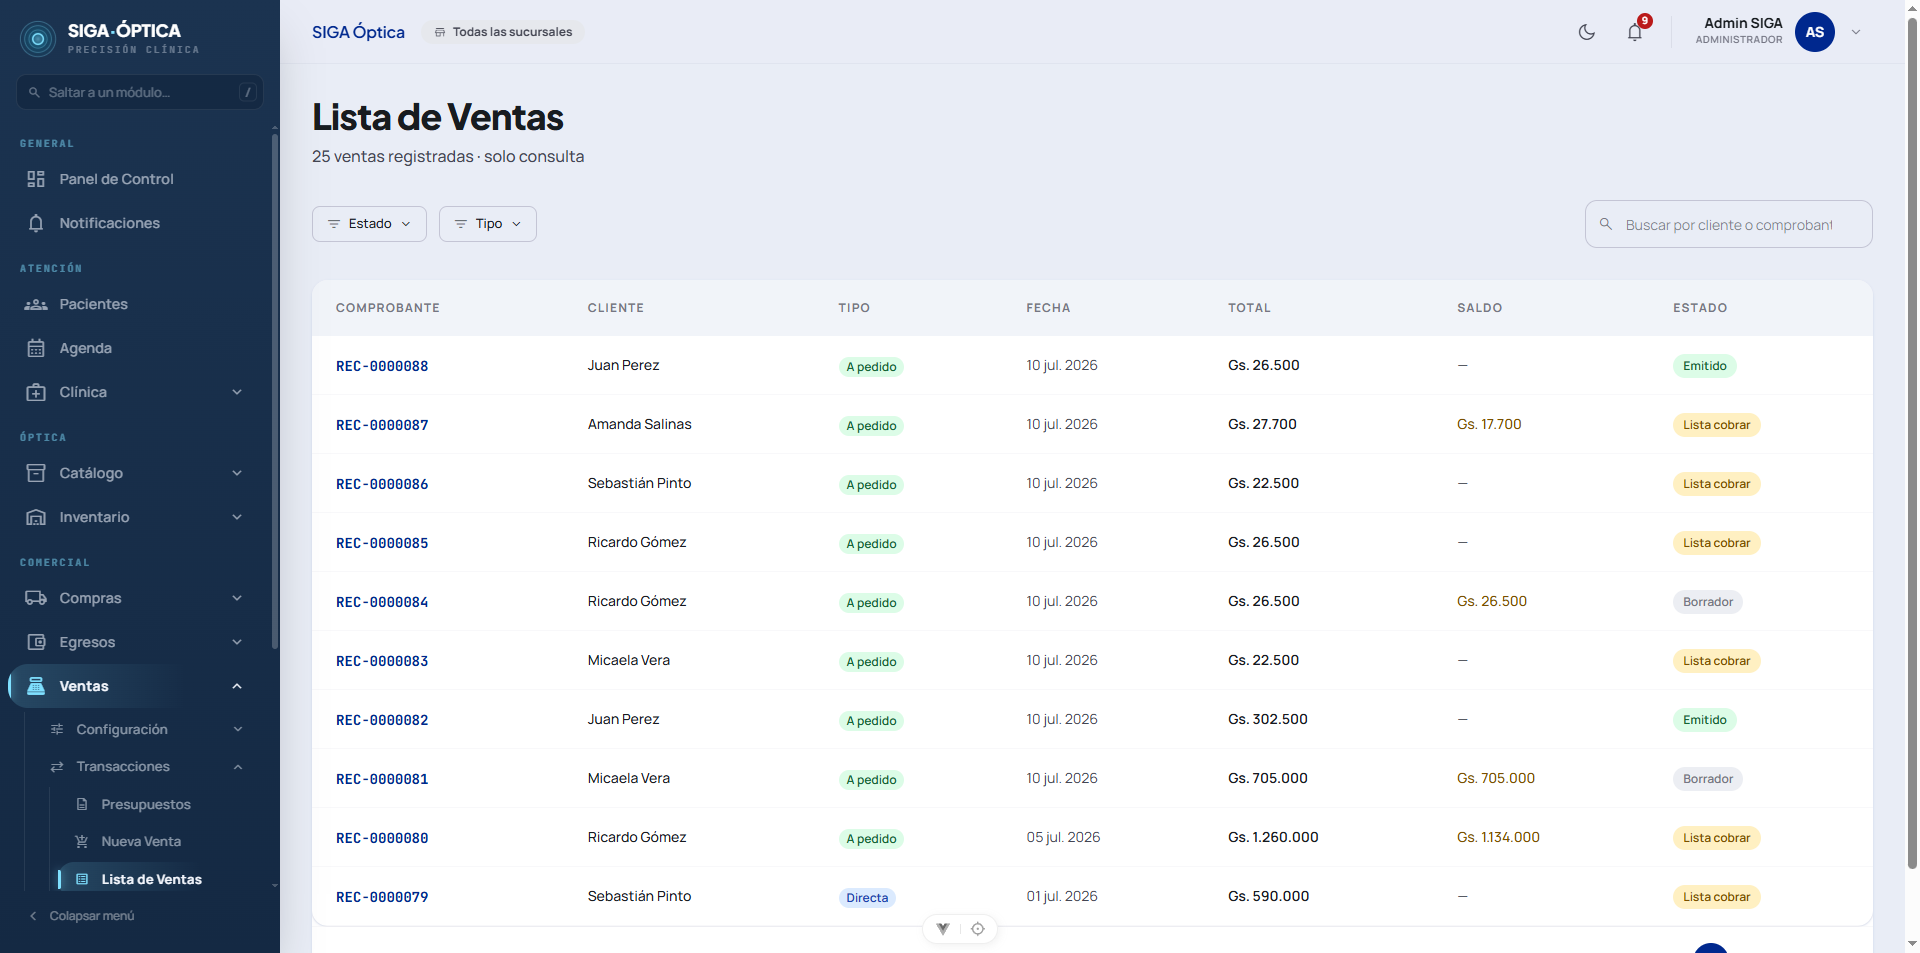
\includegraphics[width=0.95\textwidth]{imagenes/mod08-ventas.png}
\caption{Listado de ventas, con tipo (directa o a pedido), total, saldo pendiente y estado de cada una.}
\label{fig:mod08-ventas}
\end{figure}

\section{Estado}
\label{sec:08-estado}

\Implementado\ y en uso, con dos particularidades a tener en cuenta:
\begin{itemize}
  \item El flujo de ``generar venta desde presupuesto'' carga líneas más cliente más receta y confirma, pero \textbf{no rehidrata} la \code{TrabajoOpticoCard} (la config óptica ya quedó fija en el \code{TrabajoPedido} del presupuesto) --- no hay endpoint para editar receta/laboratorio de un presupuesto existente al confirmarlo.
  \item \code{Venta} tiene varios totales (\code{Total}, \code{MontoSeña}, \code{TotalCobrado}, \code{SaldoPendiente}, montos por categoría fiscal) que son propiedades \textbf{calculadas en memoria} (\code{Ignore()}d por EF), no columnas --- no confundir con datos persistidos al leer el esquema.
\end{itemize}

